\documentclass[letterpaper,11pt]{article}

% Soporte para los acentos.
\usepackage[utf8]{inputenc}
\usepackage[T1]{fontenc}
% Idioma español.
\usepackage[spanish,mexico, es-tabla]{babel}
% Soporte de símbolos adicionales (matemáticas)
\usepackage{multirow}
\usepackage{amsmath}
\usepackage{amssymb}
\usepackage{amsthm}
\usepackage{amsfonts}
\usepackage{mathtools}
\usepackage{latexsym}
\usepackage{enumerate}
\usepackage{ragged2e}
\usepackage{listings}
\usepackage{xcolor}
\usepackage{graphicx}
\usepackage{hyperref}
\usepackage[caption=false]{subfig}
\newcommand{\subsubsubsection}[1]{\paragraph{#1}\mbox{}\\}
\setcounter{secnumdepth}{4}
\setcounter{tocdepth}{4}
% Modificamos los márgenes del documento.                                       %
\usepackage[lmargin=1.5cm,rmargin=1.5cm,top=1.5cm,bottom=1.5cm]{geometry}

\definecolor{codegreen}{rgb}{0,0.6,0}
\definecolor{codegray}{rgb}{0.5,0.5,0.5}
\definecolor{codepurple}{rgb}{0.58,0,0.82}
\definecolor{backcolour}{rgb}{0.95,0.95,0.92}

\lstdefinestyle{mystyle}{
    backgroundcolor=\color{backcolour},   
    commentstyle=\color{codegreen},
    keywordstyle=\color{magenta},
    numberstyle=\tiny\color{codegray},
    stringstyle=\color{codepurple},
    basicstyle=\ttfamily\footnotesize,
    breakatwhitespace=false,         
    breaklines=true,                 
    captionpos=b,                    
    keepspaces=true,                 
    numbers=left,                    
    numbersep=5pt,                  
    showspaces=false,                
    showstringspaces=false,
    showtabs=false,                  
    tabsize=2
}

\lstset{style=mystyle}

\title{Facultad de Ciencias, UNAM \\ 
       Reconocimiento de Patrones y Aprendizaje Automatizado \\ 
       GTZAN Dataset - Music Genre Classification}
\author{Rubí Rojas Tania Michelle}
\date{05 de junio de 2021}

\begin{document}
\maketitle

\section{Introducción}
Hoy en día, la música es algo indispensable para nosotros. Utilizamos 
plataformas como \texttt{Spotify}, \texttt{Youtube} o \texttt{Apple Music} 
para escuchar canciones de nuestro agrado, además de que podemos encontrar 
listas de reproducción adecuadas a nuestras preferencias o algunas otras que 
contienen canciones de acuerdo a su género musical. Éstas últimas son 
generadas automáticamente por cada plataforma, en lugar de tener a alguien 
más que las clasifique por ellos. Pero, ¿cómo lo hacen? ¿cómo logran 
automatizar este proceso? A lo largo de este trabajo lograremos ver una forma 
para lograr esto.

\section{Objetivo}
\begin{center}
    \texttt{"Dada una canción, queremos saber a qué genero musical pertenece"}
\end{center}

\section{Métodos}
\subsection{Conjunto de Datos}
El conjunto de noticias que utilizaremos se obtuvo del sitio web \textit{Kaggle}
\begin{center}
    \url{https://www.kaggle.com/andradaolteanu/gtzan-dataset-music-genre-classification}
\end{center}

el cual contiene dos archivos y dos carpetas:
\begin{enumerate}
    \item \textbf{features\_30\_sec.csv}

    Contiene $1000$ entradas ($10$ por cada género) con $60$ atributos que 
    son características basadas en el timbre, las cuales miden la similitud 
    entre canciones y proporcionan información semántica sobre la señal. Entre 
    estos atributos se encuentran:

    \begin{itemize}
        \item \textbf{filename}: el nombre del archivo.
        \item \textbf{length}: el tamaño del archivo. 
        \item \textbf{spectral\_bandwidth}: el ancho de banda espectral.
        \item \textbf{spectral\_centroid}: el centroide espectral.
        \item \textbf{rms}: el nivel promedio de una onda en el espectro.
        \item \textbf{label}: el género musical al cual pertenece.  
    \end{itemize}

    Las características brindadas en este archivo corresponden a canciones 
    cuya duración es de $30$ segundos.

    \item \textbf{features\_3\_sec.csv}

    Mismos atributos que el archivo anterior, con la diferencia de que 
    corresponden a canciones cuya duración es de $3$ segundos (por lo 
    que incrementa $10$ veces el número de entradas).

    \item \textbf{genres\_original}

    Corresponden a los audios de las canciones utilizadas en el conjunto 
    de datos.

    \item \textbf{images\_original}

    Corresponden al espectograma de Mel de cada una de las canciones 
    utilizadas en el conjunto de datos.
\end{enumerate} 

\subsection{Preprocesamiento de Datos}

Tenemos 10 géneros musicales: blues, clásica, country, disco, hiphop, jazz,
metal, pop, reggae, rock.

Los datos contenidos en el archivo \textbf{features\_3\_sec.csv} se ven de la 
siguiente forma: 
\begin{figure}[h!]
    \centering
    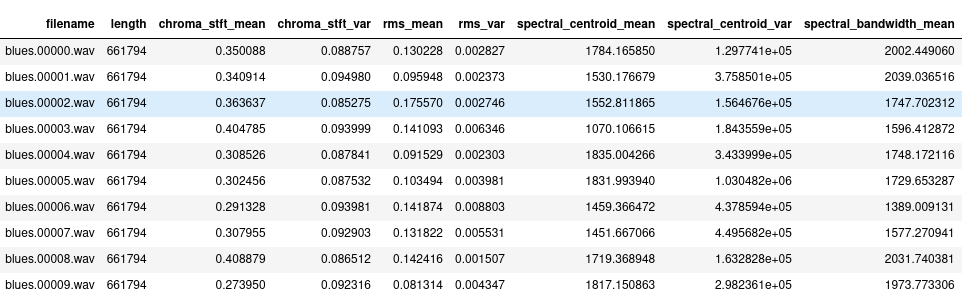
\includegraphics[width=0.9\textwidth]{imagenes/dataset.png}
    \caption{Dataset con las primeras $10$ entradas}
    \label{fig: dataframe1}
\end{figure}

Dividimos el conjunto de datos en dos:
\begin{itemize}
    \item $X$: corresponde a los primeros $59$ atributos (excepto el atributo 
    \texttt{filename}).
    
    \item $y$: corresponde al atributo $60$, el cual es la etiqueta del género 
    musical.
\end{itemize}

Normalizamos nuestro conjunto $X$ usando \texttt{StandardScaler}. Ésta clase 
estándariza los datos eliminando la media y escalando los datos de forma que 
su varianza sea igual a $1$. Ahora bien, la variable de salida es un valor de 
\texttt{string}, por lo que debemos convertirlos en valores enteros entre $0$ 
y $9$. Esto lo podemos lograr usando la clase \texttt{LabelEncoder}, pues ésta 
modelará la codificación requerida y creará una nueva variable de salida. De 
esta forma obtenemos que:
\begin{itemize}
    \item $0 \rightarrow$ blues \quad \quad \; $1 \rightarrow$ classical
    \item $2 \rightarrow$ country \quad \; $3 \rightarrow$ disco
    \item $4 \rightarrow$ hiphop \quad \quad $5 \rightarrow$ jazz 
    \item $6 \rightarrow$ metal \quad \quad \; $7 \rightarrow$ pop 
    \item $8 \rightarrow$ reggae \quad \quad $9 \rightarrow$ rock
\end{itemize}

Finalmente, dividimos nuestro conjunto de datos con un split del $80-20$ 
para entrenamiento y prueba. 

\subsection{Plan de Acción}
Para darle una solución a nuestro objetivo, utilizaremos dos \textit{modelos}
de clasificación diferentes: SVC (Support Vector Classifier) y PCA (principal 
Component Analysis) con SVC. 

\subsubsection{SVC (Support Vector Classifier)}
\subsubsubsection{Implementación}
Creamos nuestro modelo SVC (usando un kernel lineal) y lo entrenamos. Luego, 
ya podemos comenzar a realizar nuestras predicciones.

\begin{minipage}[t]{0.7\textwidth}
    \begin{lstlisting}[language = Python]
        svclassifier = SVC (kernel = 'linear')
        svclassifier . fit ( X_train, y_train)
        y_pred = svclassifier.predict(X_test)
    \end{lstlisting}
\end{minipage}

donde obtenemos un $98\%$ de precisión en el conjunto de entrenamiento y 
$76\%$ en el de prueba.

\subsubsection{PCA (principal Component Analysis) con SVC}
\subsubsubsection{Obtención del número de componentes}

Usaremos PCA para obtener la lista de atributos que tienen mayor varianza
(mayor poder explicativo). Éstos serán las componentes principales.

\begin{figure}[h]
    \centering
    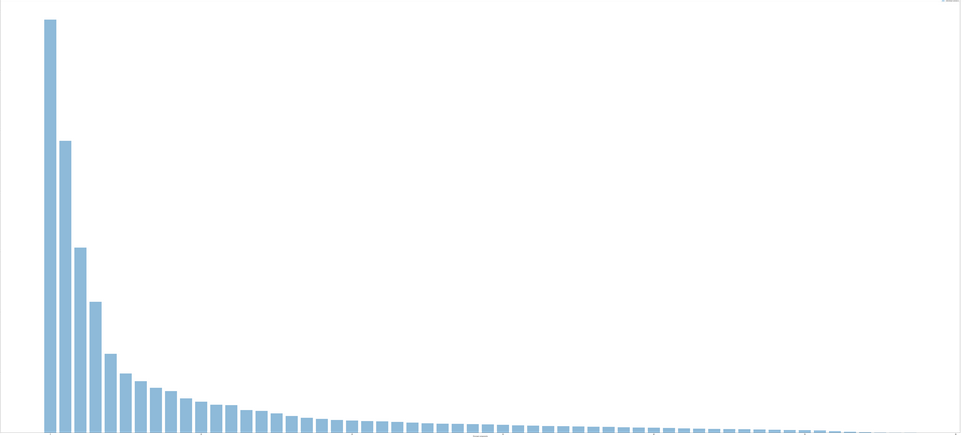
\includegraphics[width=0.8\textwidth]{./imagenes/components1.png}
    \caption{Variance ratio vs Principal components}
\end{figure}    

Con esta gráfica podemos observar que con un número de componentes entre $40$ y
$45$ se explica la mayor varianza, pero para tener un número en concreto 
realizamos además una gráfica 
\begin{center}
    \texttt{Cumulative variance vs The number of components needed to explain 
    variance}
\end{center}

la cual se encuentra en el notebook \texttt{proyecto-pca}, pero no se incluyó por 
ser demasiado grande. Gracias a esta gráfica sabemos que con $43$ componentes 
obtenemos una varianza explicada del $98\%$.

\subsubsubsection{PCA/SVC}
Creamos un modelo SVC exactamente igual que en la sección anterior, sólo que 
los datos de $X$ serán aquellos obtenidos en PCA.

Así, con este modelo obtenemos una precisión de $96\%$ en el conjunto de 
entrenamiento y $74\%$ en el conjunto de prueba. 

\newpage
\section{Resultados}

Partiéndo del hecho de que las precisiones obtenidas fueron
\begin{itemize}
    \item Para SVC: $76\%$
    \item Para PCA/SVC: $74\%$
\end{itemize}

compararemos los reportes de clasificación de ambos algoritmos.

\subsection{Reportes de clasificación}

Los reportes de clasificación muestran las principales métricas de clasificación,
incluidas la precisión y la recuperación, la puntuación (media armónica de la
precisión y la recuperación) y el soporte (número de observaciones de esa clase 
en el conjunto de entrenamiento).

\begin{figure}[ht]
    \centering
    \subfloat[SVC]
    {{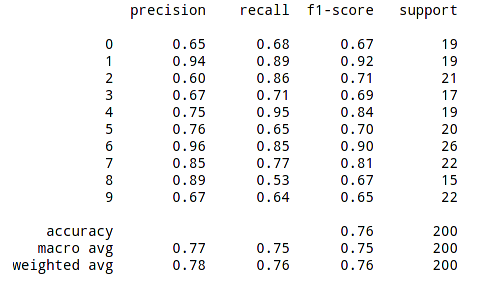
\includegraphics[width=8.5cm]{./imagenes/reporte-svd.png}}}
    \qquad
    \subfloat[PCA/SVC]
    {{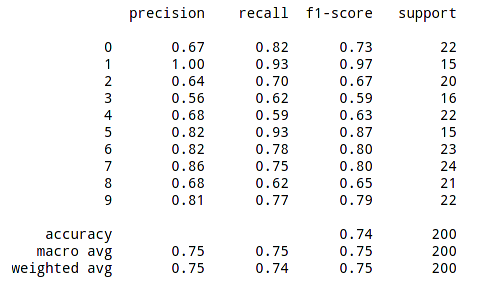
\includegraphics[width=8.5cm]{imagenes/repote-pca.png}}}
    \caption{Reportes de clasificación}
    \label{fig: reportes}
\end{figure}

Podemos notar que algunos géneros los clasificó mejor un modelo que otro.

En particular, PCA/SVC logró un mayor \textit{balance} en cuanto a las 
precisiones al momento de realizar la clasificación.

\newpage
\subsection{Predicciones}

Ahora bien, veamos cómo funciona cada uno de nuestros modelos al momento de
realizar la clasificación.

\begin{figure}[ht]
    \centering
    \subfloat[SVC]
    {{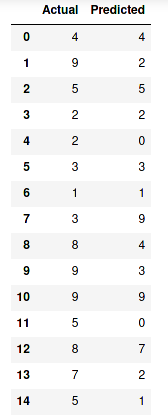
\includegraphics[width=4cm]{imagenes/svc-resultados.png}}}
    \qquad
    \subfloat[PCA/SVC]
    {{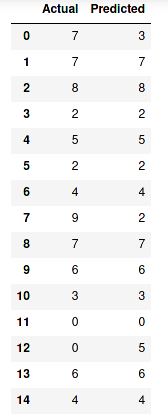
\includegraphics[width=4cm]{imagenes/pca-resultados.png}}}
\end{figure}

Para mayor simplicidad, sólo mostramos los prirmeros $15$ resultados de las 
predicciones. Como observamos, en esta primera muestra, ambos se comportan 
más o menos igual con respecto a las predicciones realizadas.

\section{Conclusiones}
Ambos modelos de clasificación me parecen bastante buenos. La precisión que se 
obtuvo en cada uno de ellos es más o menos la que esperaba, y la verdad estoy 
muy satisfecha con éstos. Me agradó el hecho de que PCA funcionara bien en 
este conjunto de datos, además de que al quitarle entre $25$ y $15$ componentes 
($95-98$ de varianza explicada), logramos obtener resultados considerablemente 
buenos al momento de la clasificación. Al final me quedé con $43$ componentes, 
pues así obtenía un valor de precisión que me agradaba más. 

Mi principal problema al momento de elaborar el proyecto fue que tuve errores 
al momento de usar PCA. En un inicio creía que lo estaba haciéndo bien (tenía 
$20$ componentes principales), pero después de investigar un poco más, 
encontré que estaba calculando mal el número de componentes, y después de 
realizar las correcciones pertinentes, logré que PCA funcionara adecuadamente
(y esto se vio reflejado muchísimo en la precisión del nuevo modelo, pues 
pasar de $20$ a $43$ componentes es un gran cambio).

Respecto al proyecto en general, siento que la elección del tema me ayudó mucho 
a comprender y reforzar algunos otros aspectos. Un \texttt{dataset} de música 
me amenizó la realización del proyecto, pues era algo que me llamaba mucho la 
atención y la clasificación de música es algo del diario en las plataformas 
digitales. Creo que el paso siguiente es realizar un sistema recomendador de 
música utilizándo redes neuronales, el cual es un proyecto que haré en mi 
tiempo libre.

\newpage
\begin{thebibliography}{9} 
    \bibitem{1} 
    SVC lineal \\
    \url{https://unipython.com/svc-lineal-machine-learning/}

    \bibitem{2}
    Implementing SVM and Kernel SVM with Python's Scikit-Learn \\ 
    \url{https://stackabuse.com/implementing-svm-and-kernel-svm-with-pythons-scikit-learn/}

    \bibitem{3}
    Dimensionality Reduction in Python with Scikit-Learn \\ 
    \url{https://stackabuse.com/dimensionality-reduction-in-python-with-scikit-learn/}
\end{thebibliography}
\end{document}
